\documentclass[hidelinks]{ctexart}

\usepackage[sensei=程光磊,gakka=原子物理学,section=Ryoushirikigaku,gakkabbr=AP]{styles/kurisu}
\usepackage{van-de-la-illinoise}

\begin{document}

\section{晶体结构} % (fold)
\label{sec:晶体结构}

\subsection{Bravais Lattice} % (fold)
\label{sub:bravais_lattice}

\subsubsection{晶格} % (fold)
\label{ssub:晶格}

\begin{ex}
    \ce{CsCl}视为一简单立方晶格上叠加\ce{CsCl}结构.
\end{ex}
Bravais格子标记晶体的平移对称性.
\begin{ex}
    六边形密铺的Primitive cell是一平行四边形, 由两个原子构成.
\end{ex}

% subsubsection 晶格 (end)

\subsubsection{数学表示} % (fold)
\label{ssub:数学表示}

Bravais格子可视为由
\[ \+vR_n = n_1 \+va_1 + n_2 \+va_2 + n_3 \+va_3 \]
所代表的全部点的集合. 其中$\curb{\+va_1,\+va_2,\+va_3}$是一组非退化矢量, 谓Bravais格子的基矢(primitive vector). $\+vR_n$谓Bravais格子的格矢, 其端点谓格点(lattice site).
\par
最小的重复单元谓点阵的原胞(\gloss{primitive cell}). 二维情形下为平行四边形, 三维情形下为parallelepiped, 体积为
\[ V = \+va_1 \cdot \+va_2 \times \+va_3. \]
\par
\gloss{Conventional cells}是人们约定能够反映对称性特点的单位. 其可能并非原胞, 但提体积一定是原胞的整数倍.
\par
原胞中只含有一个格点, 但不一定只有一个原子. 原胞的选取并非唯一.

% subsubsection 数学表示 (end)

\subsubsection{Wigner-Seitz原胞} % (fold)
\label{ssub:wigner_seitz原胞}

选定一个格点, 作其与其它各个格点的中垂线/中垂面, 其所围成之区域为\gloss{Wigner-Seitz}原胞.

% subsubsection wigner_seitz原胞 (end)

\subsubsection{常见格子} % (fold)
\label{ssub:常见格子}

\paragraph{SC} % (fold)
\label{par:sc}

Primitive cell为正方体. 配位数$6$.

% paragraph sc (end)

\paragraph{BCC} % (fold)
\label{par:bcc}

WS primitive cell为截角八面体. 配位数为$8$. 可能的基矢为
\[ \begin{pmatrix}
    1/2 \\ 1/2 \\ -1/2
\end{pmatrix},\quad \begin{pmatrix}
    -1/2 \\ 1/2 \\ 1/2
\end{pmatrix},\quad \begin{pmatrix}
    1/2 \\ -1/2 \\ 1/2
\end{pmatrix}. \]

% paragraph bcc (end)

\paragraph{FCC} % (fold)
\label{par:fcc}

WS primitive cell为正十二面体. 配位数为$12$. 可能的基矢为
\[ \begin{pmatrix}
    0 \\ 1/2 \\ -1/2
\end{pmatrix},\quad \begin{pmatrix}
    1/2 \\ 0 \\ 1/2
\end{pmatrix},\quad \begin{pmatrix}
    1/2 \\ 1/2 \\ 0
\end{pmatrix}. \]

% paragraph fcc (end)

\paragraph{简单六角} % (fold)
\label{par:简单六角}

WS primitive cell为六角棱柱. $xy$平面内配位数为$6$.

% paragraph 简单六角 (end)

一共有$14$种Bravais lattice, $7$大晶系.

% subsubsection 常见格子 (end)

\subsubsection{晶面, 晶向及其标志} % (fold)
\label{ssub:晶面_晶向及其标志}

设某一方向上阵点到最近一个阵点的位移矢量为
\[ l_1 \+va_1 + l_2 \+va_2 + l_3 \+va_3 \]
则晶向用$\brac{l_1l_2l_3}$表示.
\begin{sample}
    \begin{ex}
        简单立方晶格的$OA$方向记作$\brac{100}$, 其反方向记作$\brac{\conj{1}00}$, 其等效方向($6$个)记作$\expc{100}$. 同样, $\expc{111}$代表$8$个体对角线晶向, 而$\expc{110}$由$4$个等效方向组成.
    \end{ex}
\end{sample}
\par
晶面指数(\gloss{Miller index})的确定方法:
\begin{cenum}
    \item 任取一晶面, 以$a,b,c$为单位测量其在三个轴上的截距.
    \item 写出三个截距的倒数, 当和一个坐标轴平行时相应的倒数为零.
    \item 将三个倒数之比化为最简整数比, 以圆括号括起, 形如$\pare{hkl}$.
\end{cenum}
等效晶面用$\curb{hkl}$表示.
\begin{remark}
    晶面指数全部取反确定的晶面系不变.
\end{remark}
\begin{remark}
    若三个基矢长度相等, 晶面指数恰好为法线方向与三个坐标轴的方向余弦之比.
\end{remark}
\begin{remark}
    简单立方晶格中, Miller指数和晶面法向指数相同.
\end{remark}
\begin{remark}
    Planes of low indices are more wildly spaced, while planes of high indices are less wildly spaces. 
\end{remark}
In fcc and bcc lattice, the indices are relative to the conventional cells instead of the primitive cells.

% subsubsection 晶面_晶向及其标志 (end)

% subsection bravais_lattice (end)

\subsection{对称性} % (fold)
\label{sub:对称性}

\gloss{对称操作}是维持整个物体不变进行的操作. \gloss[\baselineskip]{点对称操作}维持至少一点保持不变. \gloss[\baselineskip]{对称元素}是对称操作过程中保持不变的集合要素, 例如点, 反演中心; 面, 反映面.
\par
保持两个矢量内积不变的线性变换是$O\pare{3}$变换. 例如Inversion对应的矩阵为
\[ \begin{pmatrix}
    -1 & & \\
    & -1 & \\
    & & -1
\end{pmatrix}, \]
reflection (mirror)对应的矩阵为
\[ \begin{pmatrix}
    0 & & \\
    & 0 & \\
    & & -1
\end{pmatrix}. \]
\begin{sample}
    \begin{ex}
        立方体可以绕$4$个体对角线旋转$\pm 2\pi/3$, 共$8$个对称操作. 绕$3$个立方轴可以旋转$\pm \pi/2, \pi$, 共$9$个对称操作, 绕$6$条棱对角线可以转动$\pi$, 共$6$个对称操作, 加上反演一共$48$个.
    \end{ex}
\end{sample}
\begin{sample}
    \begin{ex}
        将正四面体放入立方体. 可以发现绕立方轴转$\pi$, 绕体对角线转$\pm 2\pi/3$, 可以发现$12$个对称操作. 将绕棱对角线转$\pi$, 加上中心反演, 又可以产生$12$种. 凡$24$种.
    \end{ex}
\end{sample}
\begin{sample}
    \begin{ex}
        正六角柱有绕中心轴转动的$5$个非单位对称操作, 绕对棱中心连线转$\pi$和绕相对面中心连线转$\pi$, 发现$12$个. 每个操作可以附加中心反演, 一共$24$个.
    \end{ex}
\end{sample}
对称元素可以按照如下记号指定:
\begin{cenum}
    \item 绕某个轴有$n$重转动对称性, 记作$n$;
    \item 绕某个轴旋转$2\pi/n$的倍数后反演不变, 则谓之$n$重旋转-反演轴, 记作$\conj{n}$;
    \item inversion记作$i$.
\end{cenum}
\begin{sample}
    \begin{ex}
        立方体的对称元素有$1,2,3,4,i,\conj{2},\conj{3},\conj{4}$.
    \end{ex}
\end{sample}
\begin{theorem}
    晶体中允许的转动对称轴只能是$1,2,3,4$和$6$重轴.
\end{theorem}
\begin{theorem}
    晶体中允许的宏观对称性只有$1,2,3,4,6,i,m,\conj{4}$.
\end{theorem}
有些对称素可以通过其它对称素组合给出. 例如$\conj{2} = m$, $\conj{3} = 3\cup i$而$\conj{6}=3\cup m$.

\subsubsection{点群} % (fold)
\label{ssub:点群}

\gloss{点群}是点对称操作基础上组成的对称操作群.
\begin{ex}
    若晶体中存在两个两重轴, 则它们之间的夹角只能是$\SI{30}{\degree}$, $\SI{45}{\degree}$, $\SI{60}{\degree}$或$\SI{90}{\degree}$.
\end{ex}
点群通常使用Sch\"onflies符号. $C_n$表示存在$n$次转轴, $S_n$表示存在$n$次旋转-反演轴, $D_n$表示$n$次旋转轴加上与之垂直的二次轴. $T$表示四面体群, $O$表示八面体群. $h$下表表示对称与$n$次轴的水平面为对称面, $v$表示含有$n$次轴的平面为对称面, $d$表示垂直于主轴的两个二次轴的平分面为对称面.
\par
一共有$7$种晶系, $14$种格子, $32$种点群.

% subsubsection 点群 (end)

\subsubsection{空间群} % (fold)
\label{ssub:空间群}

一共有$230$种空间群. 考虑到空间对称性后, 允许的空间操作为
\begin{cenum}
    \item 平移操作与平移轴;
    \item 螺旋旋转与螺旋轴;
    \item 滑移反映与滑移面.
\end{cenum}
\begin{sample}
    \begin{ex}
        在金刚石结构中存在一个螺旋轴.
    \end{ex}
\end{sample}
\begin{sample}
    \begin{ex}
        氯化钠中存在一个滑移对称性. 氯化钠的点群为$O_h$(钠处在氯组成的八面体中心).
    \end{ex}
\end{sample}

% subsubsection 空间群 (end)

\subsubsection{对称操作与张量} % (fold)
\label{ssub:对称操作与张量}

在坐标变换$x' = Ax$下张量的变化为$T' = ATA^{-1} = ATA^T$. 若$A$为晶体的对称变换则$T=ATA^T$, 由此可得$T$的分量之间的关系.
\begin{ex}
    取$A$为绕$x$轴转$\pi$和绕$z$轴转$\pi/2$可得立方晶体中的介电张量具有可约化为一介电常数.
\end{ex}

% subsubsection 对称操作与张量 (end)

% subsection 对称性 (end)

\subsection{典型结构} % (fold)
\label{sub:典型结构}

\subsubsection{密排} % (fold)
\label{ssub:密排}

原子排列最紧密的平面谓\gloss{密排面}. ABABAB型排列给出HCP排列, ABCABC型排列给出FCC结构, 密排面为$\pare{111}$面. 两者的配位数皆为$12$.
\begin{pitfall}
    HCP并非Bravais格子.
\end{pitfall}

% subsubsection 密排 (end)

\subsubsection{简写} % (fold)
\label{ssub:简写}

\begin{cenum}
    \item 元素晶体:
    \begin{cenum}
        \item A1: 例如\ce{Cu}, FCC;
        \item A2: 例如\ce{W}, BCC;
        \item A3: 例如\ce{Mg}, HCP;
        \item A4: 金刚石.
    \end{cenum}
    \item \ce{AB}型化合物:
    \begin{cenum}
        \item B1: \ce{NaCl};
        \item B2: \ce{CsCl};
        \item B3: 闪锌矿\ce{ZnS}, FCC叠加, 类似金刚石;
        \item B4: 纤锌矿, 两个HCP的嵌套.
    \end{cenum}
    \item \ce{AB2}型化合物:
    \begin{cenum}
        \item C1: 萤石与反萤石结构(\ce{CaF2});
        \item C2: 黄铁矿(\ce{FeS2});
        \item C3: 赤铜矿(\ce{Cu2O}).
    \end{cenum}
    \item 三元化合物:
    \begin{cenum}
        \item E: Perovskite, 钙钛矿结构.
    \end{cenum}
\end{cenum}

% subsubsection 简写 (end)

\subsubsection{二维情形} % (fold)
\label{ssub:二维情形}

$10$个点群, $4$个晶系, $5$种Bravais格子.
\begin{sample}
    \begin{ex}
        在FCC结构中, $\pare{100}$表面具有$4$重旋转对称性, $\pare{110}$表面具有$2$重旋转对称性, $\pare{111}$表面具有$3$重旋转对称性.
    \end{ex}
\end{sample}

\paragraph{Wood Notation} % (fold)
\label{par:wood_notation}

用以标记表面重构.

% paragraph wood_notation (end)

% subsubsection 二维情形 (end)

% subsection 典型结构 (end)

\subsection{Reciprocal Lattice and Brillouin Zones} % (fold)
\label{sub:reciprocal_lattice_and_brillouin_zones}

\subsubsection{Definition} % (fold)
\label{ssub:definition}

The \gloss{reciprocal lattice} is defined by the basis vectors $\pare{\+vb_1,\+vb_2,\+vb_3}$ that satisfy
\[ \+va_i \cdot \+vb_j = 2\pi \delta_{ij}. \]
The reciprocal lattice consists of the translation vectors
\[ \+vG_{hkl} = h\+vb_1 + k\+vb_2 + l\+vb_3. \]
\begin{remark}
    The basis vectors $\+vb_i$ may be defined by the inverse matrix of $\pare{\+va_i}$.
\end{remark}
Some properties of the reciprocal lattice are
\begin{cenum}
    \item $\+va_i \cdot \+vb_j$ = $2\pi \delta_{ij}$;
    \item $\+vG \cdot \+vR = 2\pi \pare{n_1h_1 + n_2h_2 + n_3 h_3}$;
    \item $\displaystyle V\+_rec_ = \frac{\pare{2\pi}^3}{V}$;
    \item Surfaces $\pare{h_1h_2h_3}$ are perpendicular to $\+vG_{h_1h_2h_3}$. And
    \[ d_{h_1h_2h_3} = \frac{2\pi}{\abs{\+vG_{h_1h_2h_3}}}. \]
    \item 倒易点阵的倒格子是正点阵.
    \item 同一晶格的正格子和倒格子具有相同的对称性.
\end{cenum}
晶面取向和间距可以直接用倒格子中的一个点表示出来. 指数小的晶面系间距大.
\par
Lattice planes may be represented by
\[ \resumath{\+vG_{h_1h_2h_3}\cdot \+vr = 2\pi n.} \]
The \gloss{First Brillouin Zone} is the Wigner-Seitz cell of the reciprocal lattice.\par
Brillouin Zone的界面上的矢量$\+vk$满足
\[ \+vk\cdot \+vG = \half G^2, \]
其中$\+vG$是该界面作为垂直平分面对应的格点.
\begin{remark}
    以次近邻为第二BZ, 以此类推. 每个BZ的体积相等. 非First BZ可以通过平移填满First BZ.
\end{remark}

% subsubsection definition (end)

\subsubsection{物理意义} % (fold)
\label{ssub:物理意义}

A function $F\pare{\+vr}$ that satisfies $F\pare{\+vr+\+vR_n} = F\pare{\+vr}$ may be expanded into Fourier series as
\[ \+vF\pare{\+vr} = \sum_k A\pare{\+vk}\exp\pare{i\+vk\cdot \+vr}, \]
where
\[ A\pare{\+vk} = \rec{\Omega}\int_\Omega \rd{\+vr}\, F\pare{\+vr}\exp\pare{-i\+vk\cdot \+vr}. \]
$A\pare{\+vk}$ is invariant under $\+vr \rightarrow \+vr+\+vR_n$, therefore
\[ A\pare{\+vk} = A\pare{\+vk} \exp\pare{i\+vk\cdot \+vR_n} \Rightarrow \+vk = \+vG_{h_1h_2h_3}. \]
Hence
\[ \resumath{F\pare{\+vr} = \sum_{\+vk \in \+vG} A\pare{\+vk} \exp\pare{i\+vk\cdot \+vr}.} \]

% subsubsection 物理意义 (end)

\subsubsection{例子} % (fold)
\label{ssub:例子}

\paragraph{2D Crystals} % (fold)
\label{par:2d_crystals}

$\+vb_1$ and $\+vb_2$ are obtained by rotating $\+va_2$ and $\+va_1$ by \SI{90}{\degree}, respectively, with proper normalization.

% paragraph 2d_crystals (end)

\paragraph{Hexagonal} % (fold)
\label{par:hexagonal}

The reciprocal lattice of the hexagonal lattice is another hexagonal lattice lattice.

% paragraph hexagonal (end)

\paragraph{SC} % (fold)
\label{par:sc}

The reciprocal lattice of the SC is another SC lattice, where $a\rightarrow 2\pi/a$.
\begin{figure}[ht]
    \centering
    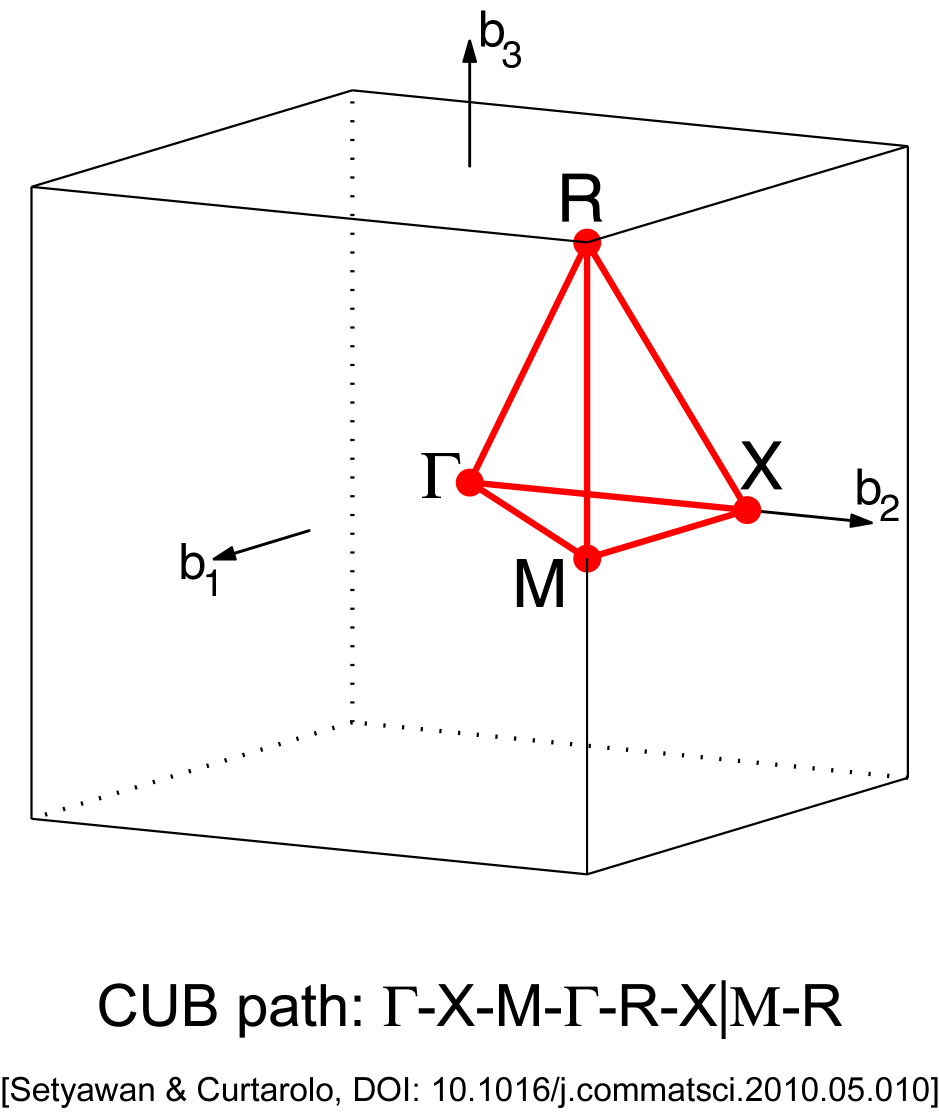
\includegraphics[width=.3\textwidth]{src/SCBZ.png}\\
    $\Gamma: \pare{0,0,0}$, $\displaystyle X:\pare{\frac{\pi}{a},0,0}$, $\displaystyle  M: \pare{\frac{\pi}{a},\frac{\pi}{a},0}$, $\displaystyle R: \pare{\frac{\pi}{a},\frac{\pi}{a},\frac{\pi}{a}}$
    \caption{The reciprocal lattice and the first BZ of the SC.}
\end{figure}

% paragraph sc (end)

\paragraph{BCC} % (fold)
\label{par:bcc}

The reciprocal lattice of the BCC is a FCC lattice.
\begin{figure}[ht]
    \centering
    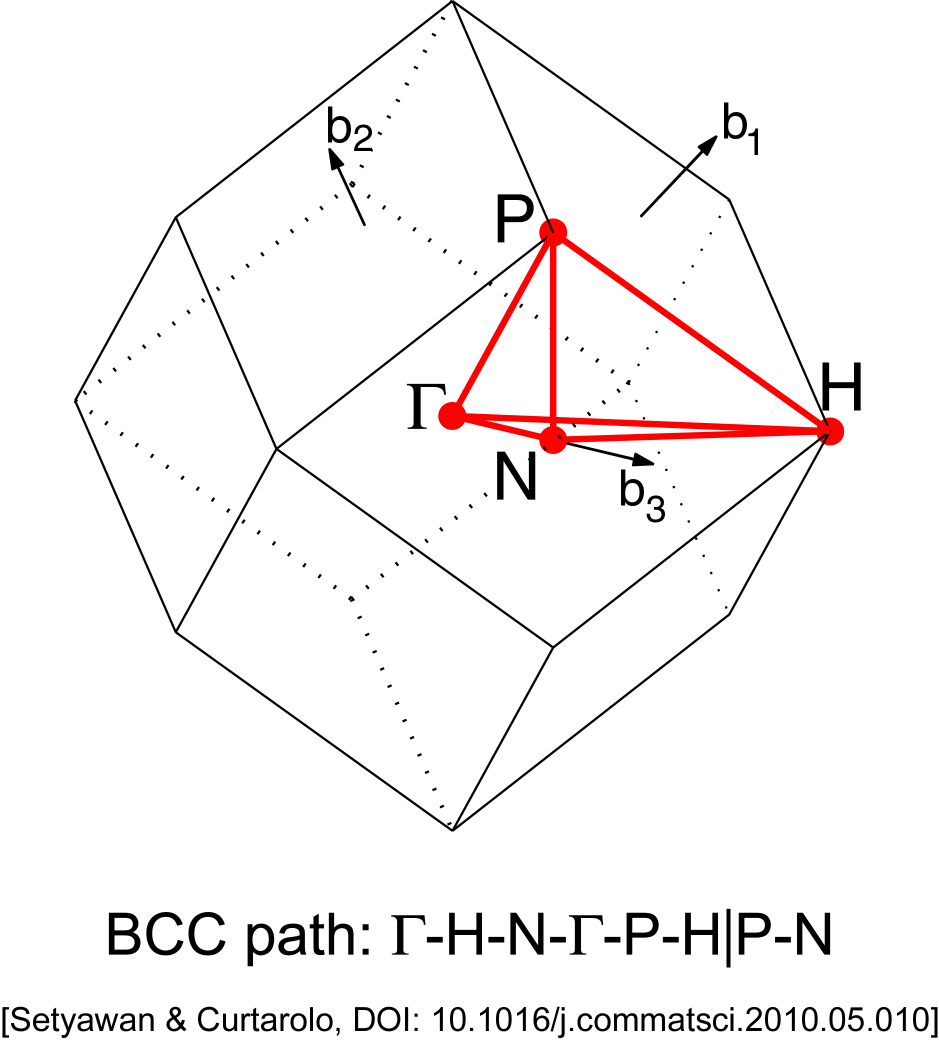
\includegraphics[width=.3\textwidth]{src/BCCBZ.png}
    \caption{The reciprocal lattice and the first BZ of the BCC, which is also the Wigner-Seitz cell of the FCC lattice.}
\end{figure}

% paragraph bcc (end)

\paragraph{FCC} % (fold)
\label{par:fcc}

The reciprocal lattice of the FCC is a BCC lattice, where $a\rightarrow 4\pi/a$.
\begin{figure}[ht]
    \centering
    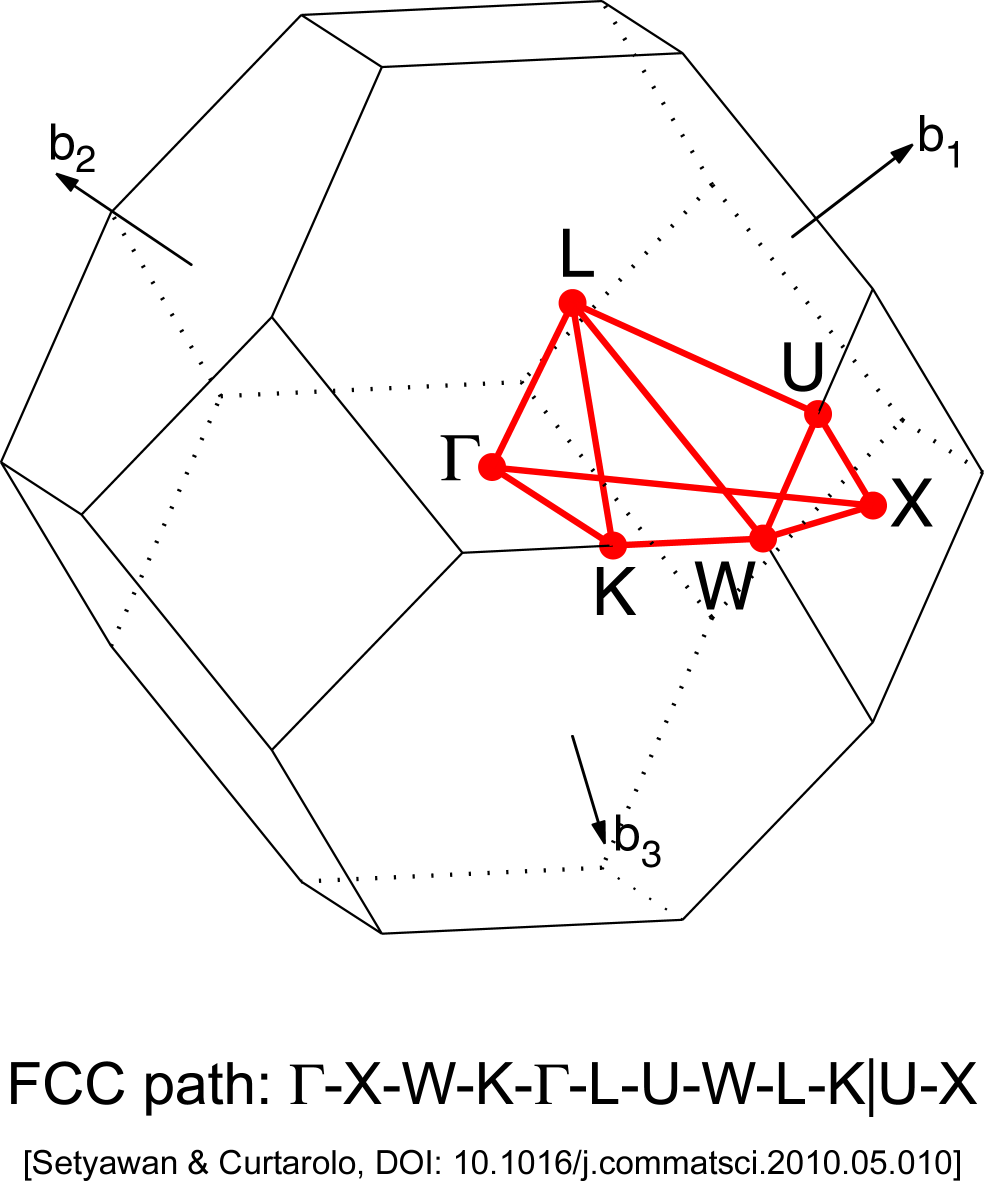
\includegraphics[width=.3\textwidth]{src/FCCBZ.png}
    \caption{The reciprocal lattice and the first BZ of the FCC, which is also the Wigner-Seitz cell of the BCC lattice.}
\end{figure}

% paragraph fcc (end)

% subsubsection 例子 (end)

% subsection reciprocal_lattice_and_brillouin_zones (end)

\subsection{Experimental Methods} % (fold)
\label{sub:experimental_methods}

\subsubsection{XRD} % (fold)
\label{ssub:xrd}

\paragraph{Lattice} % (fold)
\label{par:lattice}

衍射峰出现在满足Bragg条件
\[ \resumath{2d_{hkl}\sin\theta = n\lambda} \]
处. 将Bragg条件平方代入不同晶系的晶面间距可得其衍射$\theta$样式.
\par
Laue条件要求
\[ \+vR_n\cdot \pare{\+vn\+_incident_ - \+vn\+_diffraction_} = n\lambda, \]
从而
\[ \resumath{\+vk\+_incident_ - \+vk\+_diffraction_ = \+vG_{hkl},} \]
which may be rewritten as
\[ \+vk\cdot \+vG_{hkl} = \half \+vG_{hkl}^2. \]
Laue衍射条件等同于要求$\+vk$处于Brillouin Zone的边界.

% paragraph lattice (end)

\paragraph{Ewald球图解法} % (fold)
\label{par:ewald球图解法}

将入射波矢的起点移动到$\+vG$的原点. 以入射波矢端点为圆心, 以$k$为半径作反射球, 由$\+vk$的端点向落在球面上的倒格点引出波矢, 则其满足Bragg条件.

% paragraph ewald球图解法 (end)

\paragraph{影响衍射强度的因素} % (fold)
\label{par:影响衍射强度的因素}

原子的相干散射振幅和电子的散射振幅之比为\gloss{原子散射因子}. 若一个晶胞内有多个原子, 则一个原胞内原子的相干散射振幅与电子的散射振幅值比为\gloss{晶胞几何结构因子},
\[ S_{\+vG} = \sum_j f_j \exp\pare{-i\+vG\cdot \+vr_j} = \sum_j f_j \exp\brac{-2\pi i\pare{h_1 x_j + h_2 y_j + h_3 z_j}}, \]
\begin{sample}
    \begin{ex}
        BCC的结构因子为
        \[ S_{\+vG} = \begin{cases}
            0, & \text{$h_1+h_2+h_3$为奇数}, \\
            2f, & \text{$h_1+h_2+h_3$为偶数},
        \end{cases} \]
        因此只有$h_1+h_2+h_3$为偶数的时才会出现衍射斑.
    \end{ex}
\end{sample}
\begin{sample}
    \begin{ex}
        FCC结构的衍射因子为
        \[ S_{\+vG} = f\curb{1+\exp\brac{-i\pi\pare{h_2+h_3}} + \exp\brac{-i\pi\pare{h_1+h_3}} + \exp\brac{-i\pi\pare{h_1+h_2}} }. \]
        因此只有当$h_1$, $h_2$, $h_3$全部为偶数或奇数时, 才会出现衍射斑.
    \end{ex}
\end{sample}

% paragraph 影响衍射强度的因素 (end)

% subsubsection xrd (end)

% subsection experimental_methods (end)

% section 晶体结构 (end)

\end{document}
